%% AMS-LaTeX Created with the Wolfram Language : www.wolfram.com

\documentclass{article}
\usepackage{amsmath, amssymb, graphics, setspace}

\newcommand{\mathsym}[1]{{}}
\newcommand{\unicode}[1]{{}}

\newcounter{mathematicapage}
\begin{document}

\title{The Principle of Least Action}
\author{Jason Gross, December 7, 2010\\
Last Updated September 23, 2023}
\date{}
\maketitle

\section*{Introduction}

Recall that we defined the \textit{ Lagrangian} to be the kinetic energy less potential energy, \(L=K-U\), at a point. { }The action is then defined
to be the integral of the Lagrangian along the path,

\[S=\int_{t_0}^{t_1} L \, dt=\int _{t_0}^{t_1}K-Udt\]

It is (remarkably!) true that, in any physical system, the path an object actually takes minimizes the action. { }It can be shown that the extrema
of action occur at

\[\frac{\partial L}{\partial q}-\frac{d}{dt}\frac{\partial L}{\partial \dot{q}}=0\]

This is called the Euler equation, or the Euler-Lagrange Equation.

\subsection*{Derivation}

Courtesy of Scott Hughes{'}s Lecture notes for 8.033. { }(Most of this is copied almost verbatim from that.)

Suppose we have a function \(f\left(x,\dot{x};t\right)\) of a variable \(x\) and its derivative \(\dot{x}=dx/dt\). { }We want to find an extremum
of 

\[J=\int_{t_0}^{t_1} f\left(x(t),\dot{x}(t);t\right) \, dt\]

Our goal is to compute \(x(t)\) such that \(J\) is at an extremum. { }We consider the limits of integration to be fixed. { }That is, \(x\left(t_1\right)\)
will be the same for any \(x\) we care about, as will \(x\left(t_2\right)\).

Imagine we have some \(x(t)\) for which \(J\) is at an extremum, and imagine that we have a function which parametrizes how far our current path
is from our choice of \(x\):

\[x(t;\alpha )=x(t)+\alpha  A(t)\]

The function \(A\) is totally arbitrary, except that we require it to vanish at the endpoints: \(A\left(t_0\right)=A\left(t_1\right)=0\). { }The
parameter \(\alpha\) allows us to control how the variation \(A(t)\) enters into our path \(x(t;\alpha )\).

The {``}correct{''} path \(x(t)\) is unknown; our goal is to figure out how to construct it, or to figure out how \(f\) behaves when we are on it.

Our basic idea is to ask how does the integral \(J\) behave when we are in the vicinity of the extremum. { }We know that ordinary functions are flat
--- have zero first derivative --- when we are at an extremum. { }So let us put

\[J(\alpha )=\int_{t_0}^{t_1} f\left(x(t;\alpha ),\dot{x}(t;\alpha );t\right) \, dt\]

We know that \(\alpha =0\) corresponds to the extremum by definition of \(\alpha\). { }However, this doesn{'}t teach us anything useful, sine we
don{'}t know the path \(x(t)\) that corresponds to the extremum.

But we also know We know that \(\left.\frac{\partial J}{\partial \alpha }\right| _{\alpha =0}=0\) since it{'}s an extremum. { }Using this fact,

\[\frac{\partial J}{\partial \alpha }=\int_{t_0}^{t_1} \left(\frac{\partial f}{\partial x} \frac{\partial x}{\partial \alpha }+\frac{\partial f}{\partial
\dot{x}} \frac{\partial \dot{x}}{\partial \alpha }\right) \, dt\\
\\
\frac{\partial x}{\partial \alpha }=\frac{\partial }{\partial \alpha }(x(t)+\alpha  A(t))=A(t)\\
\\
\frac{\partial \dot{x}}{\partial \alpha }=\frac{\partial }{\partial \alpha }\frac{d}{dt}(x(t)+\alpha  A(t))=\frac{dA}{dt}\]

So

\[\frac{\partial J}{\partial \alpha }=\int_{t_0}^{t_1} \left(\frac{\partial f}{\partial x} A(t)+\frac{\partial f}{\partial \dot{x}}\frac{dA}{dt}\right)
\, dt\]

Integration by parts on the section term gives

\[\left.\int _{t_0}^{t_1}\frac{\partial f}{\partial \dot{x}}\frac{dA}{dt}dt=A(t)\frac{\partial f}{\partial \dot{x}}\right| _{t_0}^{t_1}-\int _{t_0}^{t_1}A(t)\frac{d}{dt}\frac{\partial
f}{\partial \dot{x}}dt\]

Since \(A\left(t_0\right)=A\left(t_1\right)=0\), the first term dies, and we get 

\[\frac{\partial J}{\partial \alpha }=\int _{t_0}^{t_1}A(t)\left(\frac{\partial f}{\partial x} -\frac{d}{dt}\frac{\partial f}{\partial \dot{x}}\right)dt\]

This must be zero. { }Since \(A(t)\) is arbitrary except at the endpoints, we must have that the integrand is zero at all points:

\[\frac{\partial f}{\partial x} -\frac{d}{dt}\frac{\partial f}{\partial \dot{x}}=0\]

This is what was to be derived.

\section*{Least action: \(F=m a\)}

Suppose we have the Newtonian kinetic energy, \(K =\frac{1}{2}m v^2\), and a potential that depends only on position, \(U=U\left(\overset{\rightharpoonup
}{r}\right)\). { }Then the Euler-Lagrange equations tell us the following:

\begin{doublespace}
\noindent\(\pmb{\text{Clear}[U,m,r]}\\
\pmb{L=\frac{1}{2} m r'[t]^2-U[r[t]];}\\
\pmb{\partial _{\{r[t]\}}L-\text{Dt}\left[\partial _{\left\{r'[t]\right\}}L,t,\text{Constants}\to m\right]==0}\)
\end{doublespace}

\begin{doublespace}
\noindent\(-U'[r[t]]-m r''[t]==0\)
\end{doublespace}

Rearrangement gives

\[-\frac{\partial U}{\partial r}=m \ddot{r} \\
\\
F=m a\]

\section*{Least action with no potential}

Suppose we have no potential, \(U=0\). { }Then \(L=K\), so the Euler-Lagrange equations become

\[\frac{\partial K}{\partial q}-\frac{d}{dt}\frac{\partial K}{\partial \dot{q}}=0\]

For Newtonian kinetic energy, \(K =\frac{1}{2}m \dot{x}^2\), this is just

\[\frac{d}{dt}m \dot{x}=0\\
\\
m \dot{x}=m v\\
\\
x=x_0+v t\]

This is a straight line, as expected.

\section*{Least action with gravitational potential}

Suppose we have gravitational potential close to the surface of the earth, \(U=m g y\), and Newtonian kinetic energy, \(K=\frac{1}{2}m \dot{y}^2\).
{ }Then the Euler-Lagrange equations become

\[-m g-\frac{d}{dt}m \dot{y}=-m g-m \ddot{y}=0\\
\\
-g=\ddot{y}\\
\\
y=y_0+a_yt-\frac{1}{2}g t^2\]

This is a parabola, as expected.

\section*{Constants of motion: Momenta}

We may rearrange the Euler-Lagrange equations to obtain

\[\frac{\partial L}{\partial q}=\frac{d}{dt}\frac{\partial L}{\partial \dot{q}}\]

If it happens that \(\frac{\partial L}{\partial q}=0\), then \(\frac{d}{dt}\frac{\partial L}{\partial \dot{q}}\) is also zero. { }This means that
\(\frac{\partial L}{\partial \dot{q}}\) is a constant (with respect to time). { }We call \(\frac{\partial L}{\partial \dot{q}}\) a (conserved) momentum
of the system.

\subsection*{Linear Momentum}

By noting that Newtonian kinetic energy, \(K =\frac{1}{2}m v^2\), is independent of the time derivatives of position, if potential energy depends
only on position, we can infer that \(\frac{\partial L}{\partial \dot{x}}\) (and, similarly, \(\frac{\partial L}{\partial \dot{y}}\) and \(\frac{\partial
L}{\partial \dot{z}}\)) are constant. { }Then \(\frac{\partial L}{\partial \dot{x}}=\frac{\partial }{\partial \dot{x}}\left(\frac{1}{2}m \dot{x}^2\right)=m
\dot{x}\). { }This is just standard linear momentum, \(m v\).

\subsection*{Angular Momentum}

Let us change to polar coordinates.

\begin{doublespace}
\noindent\(\pmb{x[\text{t$\_$}]\text{:=}r[t]\text{Cos}[\theta [t]]}\\
\pmb{y[\text{t$\_$}]\text{:=}r[t]\text{Sin}[\theta [t]]}\\
\pmb{K=\text{Expand}\left[\text{FullSimplify}\left[\frac{1}{2}m\left(x'[t]^2+y'[t]^2\right)\right]\right]\text{//}\text{TraditionalForm}}\)
\end{doublespace}

\begin{doublespace}
\noindent\(\frac{1}{2} m r'(t)^2+\frac{1}{2} m r(t)^2 \theta '(t)^2\)
\end{doublespace}

Using dot notation, this is

\begin{doublespace}
\noindent\(\pmb{K\text{/.}\text{r$\_$}'[t]\to \text{OverDot}[r]\text{/.}\text{r$\_$}[t]\to r\text{//}\text{TraditionalForm}}\)
\end{doublespace}

\begin{doublespace}
\noindent\(\frac{1}{2} \dot{\theta }^2 m r^2+\frac{m \dot{r}^2}{2}\)
\end{doublespace}

Note that \(\theta\) does not appear in this expression. { }If potential energy is not a function of \(\theta\) (is only a function of \(r\)), then
\(\frac{\partial L}{\partial \dot{\theta }}=m r^2 \dot{\theta }\) is constant. { }This is standard angular momentum, \(m r^2\omega = r m r \omega
=r\times m v\).

\section*{Classic Problem: Brachistochrone ({``}shortest time{''})}

\subsection*{Problem}

A bead starts at \(x=0\), \(y=0\), and slides down a wire without friction, reaching a lower point \(\left(x_f,y_f\right)\). { }What shape should
the wire be in order to have the bead reach \(\left(x_f,y_f\right)\) in as little time as possible.

\subsection*{Solution}

\subsubsection*{Idea}

Use the Euler equation to minimize the time it takes to get from \(\left(x_i,y_i\right)\) to \(\left(x_f,y_f\right)\).

\subsubsection*{Implementation}

Letting \(ds\) be the infinitesimal distance element and \(v\) be the travel speed,

\[T=\int_{t_i}^{t_f} \frac{ds}{v} \, dt\\
\\
ds=\sqrt{(dx)^2+(dy)^2}=dy\sqrt{1+(x')^2}\text{             }x'=\frac{dx}{dy}\\
\\
v=\sqrt{2g y}\text{             }\text{(Assumption: bead starts at rest)}\\
\\
T=\int_0^{y_f} \sqrt{\frac{1+(x')^2}{2g y}} \, dy\]

Now we apply the Euler equation to \(f=\sqrt{\frac{1+(x')^2}{2g y}}\) and change \(t\to y\), \(\dot{x}\to x'\).

\[\frac{\partial f}{\partial x}-\frac{d}{dy} \frac{\partial f}{\partial \dot{x}}=0\\
\\
\frac{\partial f}{\partial x}=0\\
\\
 \frac{\partial f}{\partial \dot{x}}=\frac{1}{\sqrt{2g y}}\frac{x'}{\sqrt{1+(x')^2}}\\
\\
\frac{d}{dy} \frac{\partial f}{\partial \dot{x}}=0\text{   }\longrightarrow \text{   }\frac{1}{\sqrt{2g y}}\frac{x'}{\sqrt{1+(x')^2}}=\text{Constant}\]

Squaring both sides and making a special choice for the constant gives

\[\frac{(x')^2}{2g y\left(1+(x')^2\right)}=\frac{1}{4 g A}\\
\\
\longrightarrow \text{     }\left(\frac{dx}{dy}\right)^2=\frac{y/(2A)}{1-y/(2A)}=\frac{y^2}{2 A y-y^2}\\
\\
\longrightarrow \text{     }x=\int_0^{y_f} \frac{dx}{dy} \, dy=\int_0^{y_f} \frac{y}{\sqrt{2 A y-y^2}} \, dy\]

To solve this, change variables:

\[y=A(1-\cos (\theta )),\text{      }dy=A \sin (\theta )d\theta\]

\begin{doublespace}
\noindent\(\pmb{\text{FullSimplify}\left[2A y-y^2\text{/.}y\to A(1-\text{Cos}[\theta ])\right]}\)
\end{doublespace}

\begin{doublespace}
\noindent\(A^2 \text{Sin}[\theta ]^2\)
\end{doublespace}

\[\frac{y}{\sqrt{2 A y-y^2}}dy=\frac{A(1-\cos (\theta ))}{\sqrt{A^2\sin ^2(\theta )}}A \sin (\theta ) d\theta =A(1-\cos (\theta ))\\
\\
x=\int_0^{\theta } A(1-\cos (\theta )) \, d\theta =A(\theta -\sin (\theta ))\]

Full solution: The brachistochrone is described by

\[\fbox{$x=A(\theta -\sin (\theta ))y=A(1-\cos (\theta ))$}\]

There{'}s no analytic solution, but we can compute them.

\begin{doublespace}
\noindent\(\pmb{\text{Clear}[x,y,A,\theta ,\text{soln},\text{yf},\text{xf},\text{xmax},\text{$\theta $max},\text{Asol},f];}\\
\pmb{\text{RepeatedFindRoot}[\text{fs$\_$},\{\theta ,\text{$\theta $0$\_$}\},\{A,\text{A0$\_$}\},\text{n$\_$}:3,\text{nMaxIterations$\_$}:\text{OptionValue}[\text{FindRoot},\text{MaxIterations}]]\text{:=}}\\
\pmb{\text{If}[n\leq 1,\text{FindRoot}[\text{fs},\{\theta ,\text{$\theta $0}\},\{A,\text{A0}\},\text{MaxIterations}\to \text{nMaxIterations}],}\\
\pmb{\text{Module}[\{\text{err},\text{soln},k=\text{Reap}[\text{Quiet}[\text{Check}[\text{Sow}[\text{RepeatedFindRoot}[\text{fs},\{\theta ,\text{$\theta
$0}\},\{A,\text{A0}\},n-1,\text{nMaxIterations}]],\text{Throw}]]]\},}\\
\pmb{\{\text{err},\{\{\text{soln}\}\}\}=k;}\\
\pmb{\text{If}[\text{SameQ}[\text{err},\text{soln}],\text{soln},\text{FindRoot}[\text{fs},\{\theta ,\text{Mod}[(\theta \text{/.}\text{soln}),2\pi
,-2\pi ]\},\{A,A\text{/.}\text{soln}\},}\\
\pmb{\text{MaxIterations}\to \text{nMaxIterations}]]]]}\\
\pmb{\text{Manipulate}[\text{Module}[\{y=\text{Function}[\{A,\theta \},A (1 - \text{Cos}[\theta ])],x =\text{Function}[\{A,\theta \}, A(\theta  -
\text{Sin}[\theta ])]\},}\\
\pmb{\text{Module}[\{\text{soln}=\text{RepeatedFindRoot}[\{x[A,\theta ]==\text{xf},y[A,\theta ]==\text{yf}\},\{\theta ,-\pi \},\{A,-1\},3,1000]\},}\\
\pmb{\text{Module}[\{\text{Asol}=A\text{/.}\text{soln},\text{$\theta $max}=\theta \text{/.}\text{soln}\},\text{ParametricPlot}[\{x[\text{Asol},\theta
],y[\text{Asol},\theta ]\},\{\theta ,0,\text{$\theta $max}\},}\\
\pmb{\text{PlotRange}\to \{\{0,\text{xmax}\},\{\text{ymax},0\}\},\text{PlotStyle}\to \text{Black}]]]],\left\{\left\{\text{xmax},2\pi ,x_{\max }\right\},0,4\pi
\right\},}\\
\pmb{\left.\left\{\left\{\text{ymax},-2.5,y_{\max }\right\},0,-20\right\},\left\{\left\{\text{xf},4,x_f\right\},1,6\right\},\left\{\left\{\text{yf},-2,y_f\right\},0,-5\right\}\right]}\)
\end{doublespace}

\begin{doublespace}
\noindent\(\fbox{$$}\)
\end{doublespace}

\section*{Classic Problem: Catenary}

\subsection*{Problem}

Suppose we have a rope of length \(l\) and linear mass density \(\lambda\). { }Suppose we fix its ends at points \(\left(x_0,y_0\right)\) and \(\left(x_f,y_f\right)\).
{ }What shape does the rope make, hanging under the influence of gravity?

\subsection*{Solution}

\subsubsection*{Idea}

Calculate the potential energy of the rope as a function of the curve, \(y(x)\), and minimize this quantity using the Euler-Lagrange equations.

\subsubsection*{Implementation}

Suppose we have curve parameterized by \(t\), \((x(t), y(t))\). { }The potential energy associated with this curve is

\[U=\int _0^l\lambda  g yds\\
\\
ds=\sqrt{(dx)^2+(dy)^2}=dy\sqrt{1+(x')^2}\text{             }x'=\frac{dx}{dy}\\
\\
U=\int _{y_0}^{y_f}\lambda  g y\sqrt{1+(x')^2}dy\]

Note that if we choose to factor \(ds\) the other way (for \(y'\)), we get a mess.

Now we apply the Euler-Lagrange equation to \(f=\lambda  g y\sqrt{1+(x')^2}\) and change \(t\to y\), \(\dot{x}\to x'\).

\[\frac{\partial f}{\partial x}-\frac{d}{dy} \frac{\partial f}{\partial x'}=0\\
\\
\frac{\partial f}{\partial x}=0\\
\\
 \frac{\partial f}{\partial x'}=\frac{\lambda  g y x'}{\sqrt{1+(x')^2}}\]

Since \(\frac{\partial f}{\partial x}=0\), \(\frac{\partial f}{\partial x'}\) is constant, say \(a= \frac{1}{\lambda  g}\frac{\partial f}{\partial
x'}=\frac{y x'}{\sqrt{1+(x')^2}}\). { }Then

\[x'=\frac{dx}{dy}=\pm \frac{a}{\sqrt{y^2-a^2}}\]

Using the fact that

\[\int \frac{dy}{\sqrt{y^2-a^2}}=\cosh ^{-1}\left(\frac{y}{a}\right)+b,\]

integration of \(x'\) gives

\[x(y)=\pm a \cosh ^{-1}\left(\frac{y}{a}\right)+b\]

where \(b\) is a constant of integration.

Plotting this for \(a=1\), \(b=0\) gives:

\begin{doublespace}
\noindent\(\pmb{\text{Clear}[y];}\\
\pmb{\text{Manipulate}\left[\text{ParametricPlot}\left[\left\{\left\{-a \text{ArcCosh}\left[\frac{t}{a}\right]+b,t\right\},\left\{a \text{ArcCosh}\left[\frac{t}{a}\right]+b,t\right\}\right\},\{t,\text{ymin},\text{ymax}\},\text{PlotStyle}\to
\text{Black},\right.\right.}\\
\pmb{\left.\text{AspectRatio}\to \text{Automatic}],\{\{a,1\},-5,5\},\{\{b,0\},-5,5\},\left\{\left\{\text{ymin},0,y_{\min }\right\},-5,5\right\},\left\{\left\{\text{ymax},2,y_{\max
}\right\},-5,5\right\}\right]}\)
\end{doublespace}

\begin{doublespace}
\noindent\(\fbox{$$}\)
\end{doublespace}

\section*{Problem: Bead on a Ring}

From 8.033 Quiz $\#$2

\subsection*{Problem}

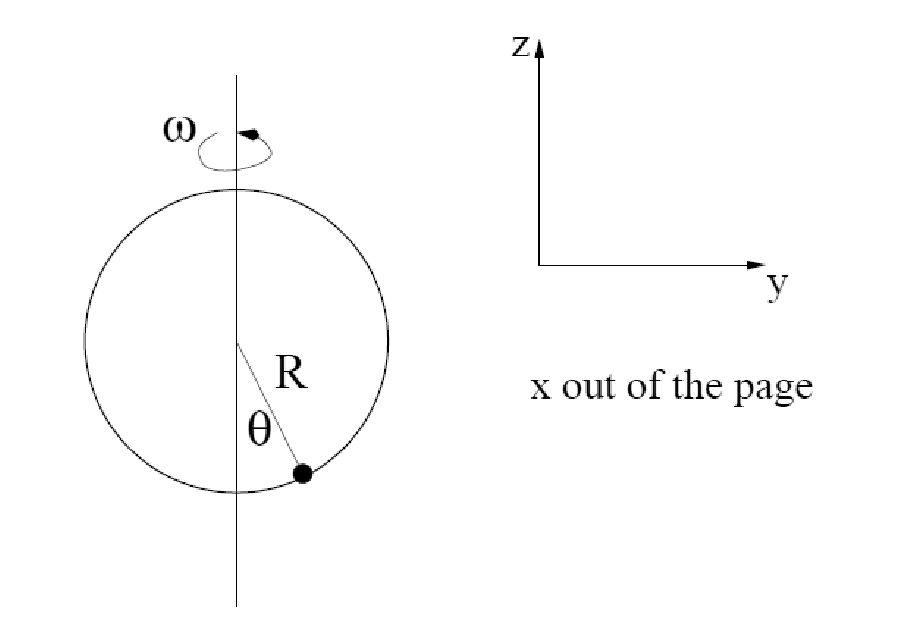
\includegraphics{Principle of Least Action_gr1.eps}

A bead of mass \(m\) slides without friction on a circular hoop of radius \(R\). The angle \(\theta\) is defined so that when the bead is at the
bottom of the hoop, \(\theta =0\). The hoop is spun about its vertical axis with angular velocity \(\omega\). Gravity acts downward with acceleration
\(g\).\\
Find an equation describing how \(\theta\) evolves with time.\\
Find the minimum value of \(\omega\) for the bead to be in equilibrium at some value of \(\theta\) other than zero.\\
({``}equilibrium{''} means that \(\dot{\theta }\) and \(\ddot{\theta }\) are both zero.) How large must \(\omega\) be in order to make \(\theta =\pi
/2\)?

\subsection*{Solution}

The general Lagrangian for the object in Cartesian coordinates is

\begin{doublespace}
\noindent\(\pmb{\text{Clear}[x,y,z,t];\left(L=\frac{1}{2}m\left(x'[t]^2+y'[t]^2+z'[t]^2\right)-m g z[t]\right)\text{//}\text{TraditionalForm}}\)
\end{doublespace}

\begin{doublespace}
\noindent\(\frac{1}{2} m \left(x'(t)^2+y'(t)^2+z'(t)^2\right)-g m z(t)\)
\end{doublespace}

Converting to polar coordinates, and using the constraints that \(\phi =\omega  t\) and \(r=R\), using the conversion

\[x=R \sin (\theta ) \cos (\omega  t)\\
\\
y=R \sin (\theta ) \sin (\omega  t)\\
\\
z=R-R \cos (\theta )\]

gives

\begin{doublespace}
\noindent\(\pmb{\text{Clear}[r,\theta ,\phi ];}\\
\pmb{\text{Defer}[L]==}\\
\pmb{(\text{Lpolar}=}\\
\pmb{\text{Expand}[\text{FullSimplify}[L\text{/.}\{x\to \text{Function}[t,R \text{Cos}[\omega  t]\text{Sin}[\theta [t]]],y\to \text{Function}[t,R
\text{Sin}[\omega  t]\text{Sin}[\theta [t]]],}\\
\pmb{z\to \text{Function}[t,R-R \text{Cos}[\theta [t]]]\}]])\text{/.}\theta '[t]\to \dot{\theta }\text{/.}\theta [t]\to \theta \text{//}\text{TraditionalForm}}\\
\pmb{0==\text{Defer}\left[\partial _{\theta }L-\text{Dt}[\text{{``}{''}},t]\partial _{\dot{\theta }}L\right]==\left(\text{EL}=\text{Expand}\left[\text{FullSimplify}\left[\partial
_{\theta [t]}\text{Lpolar}-\partial _t\partial _{\theta '[t]}\text{Lpolar}\right]\right]\right)\text{/.}\theta [t]\to \theta \text{//}\text{TraditionalForm}}\\
\pmb{\theta \text{''}[t]==(\theta \text{''}[t]\text{/.}\text{Solve}[\text{EL}==0,\theta \text{''}[t]][[1]])\text{//}\text{TraditionalForm}}\)
\end{doublespace}

\begin{doublespace}
\noindent\(L=g m R \cos (\theta )-g m R-\frac{1}{4} m R^2 \omega ^2 \cos (2 \theta )+\frac{1}{2} \dot{\theta }^2 m R^2+\frac{1}{4} m R^2 \omega ^2\)
\end{doublespace}

\begin{doublespace}
\noindent\(0=\frac{\partial L}{\partial \theta }-\frac{d\text{}}{dt} \frac{\partial L}{\partial \dot{\theta }}=-g m R \sin (\theta )+m R^2 \omega
^2 \sin (\theta ) \cos (\theta )-m R^2 \theta ''(t)\)
\end{doublespace}

\begin{doublespace}
\noindent\(\theta ''(t)=\frac{R \omega ^2 \sin (\theta (t)) \cos (\theta (t))-g \sin (\theta (t))}{R}\)
\end{doublespace}

Finding the minimum value of \(\omega\) for the bead to be in equilibrium gives

\begin{doublespace}
\noindent\(\pmb{(\theta \text{''}[t]\text{/.}\text{Solve}[\text{EL}==0,\theta \text{''}[t]][[1]])==0\text{//}\text{TraditionalForm}}\\
\pmb{\text{Refine}[\text{Reduce}[(\theta \text{''}[t]\text{/.}\text{Solve}[\text{EL}==0,\theta \text{''}[t]][[1]])==0,\text{Cos}[\theta [t]]],}\\
\pmb{\text{Sin}[\theta [t]]\neq 0\&\&R \text{Cos}[\theta [t]]\neq 0\&\&g>0\&\&R \omega \neq 0]\text{/.}\theta [t]\to \theta \text{//}\text{TraditionalForm}}\)
\end{doublespace}

\begin{doublespace}
\noindent\(\frac{R \omega ^2 \sin (\theta (t)) \cos (\theta (t))-g \sin (\theta (t))}{R}=0\)
\end{doublespace}

\begin{doublespace}
\noindent\(\cos (\theta )=\frac{g}{R \omega ^2}\)
\end{doublespace}

In order for this to have a solution, we must have 

\[\omega \geq \sqrt{\frac{g}{R}}\]

If \(\theta =\pi /2\), then \(\cos (\theta )=0\), so \(\omega =\infty\).

\section*{Problem 11.8: K $\&$ K 8.12}

\subsection*{Problem}

A pendulum is rigidly fixed to an axle held by two supports so that it can only swing in a plane perpendicular to the axle. The pendulum consists
of a mass \(m\) attached to a massless rod of length \(l\). The supports are mounted on a platform which rotates with constant angular velocity \(\Omega\).
Find the pendulum{'}s frequency assuming the amplitude is small.

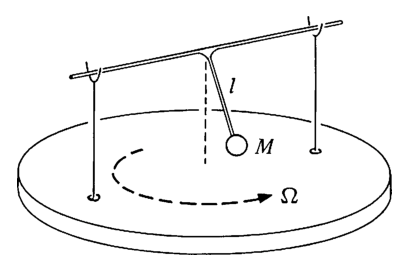
\includegraphics{Principle of Least Action_gr2.eps}

\subsection*{Solution by torque}

(From the problem set solutions)

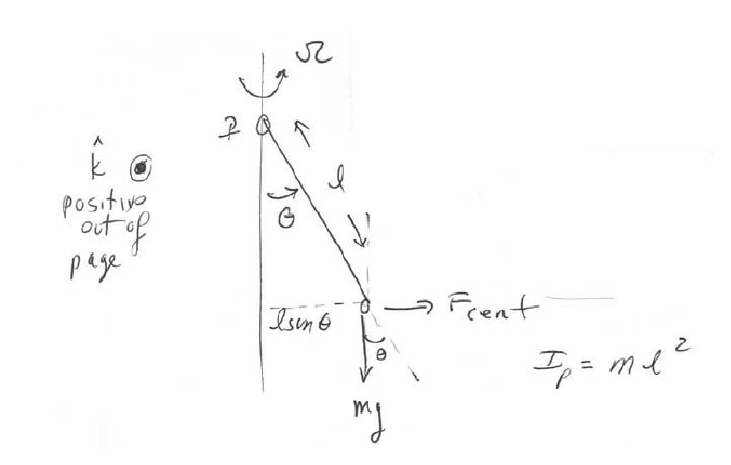
\includegraphics{Principle of Least Action_gr3.eps}

The torque about the pivot point is

\[\overset{\rightharpoonup }{\tau }_p=\overset{\rightharpoonup }{\alpha } I_p\]

\begin{equation}
\hat{k}:\text{         }-g \ell  m \sin (\theta )+\ell  F_{\text{cent}} \cos (\theta )=\ddot{\theta } I_p
\end{equation}

The centrifugal effective force is

\[F_{\text{cent}}=m (\ell  \sin (\theta ))\Omega ^2\]

For small angles, \(\sin (\theta )\simeq \theta\), \(\cos (\theta )\simeq 1\). { }Then equation (1) becomes

\[-g \ell  m \theta +m \ell ^2 \theta  \Omega ^2\simeq m \ell ^2\ddot{\theta } \\
\\
\ddot{\theta } +\left(\frac{g}{\ell }- \Omega ^2\right)\theta \simeq 0\\
\\
\omega =\sqrt{\frac{g}{\ell }-\Omega ^2}\]

If \(\Omega ^2>\frac{g}{\ell }\), the motion is no longer harmonic.

\subsection*{Solution by least action}

The general Lagrangian for the object in Cartesian coordinates is

\begin{doublespace}
\noindent\(\pmb{\text{Clear}[x,y,z,t];\left(L=\frac{1}{2}m\left(x'[t]^2+y'[t]^2+z'[t]^2\right)-m g z[t]\right)\text{//}\text{TraditionalForm}}\)
\end{doublespace}

\begin{doublespace}
\noindent\(\frac{1}{2} m \left(x'(t)^2+y'(t)^2+z'(t)^2\right)-g m z(t)\)
\end{doublespace}

Converting to polar coordinates, and using the constraints that \(\phi =\Omega  t\) and \(r=\ell\), using the conversion

\[x=\ell  \sin (\theta ) \cos (\Omega  t)\\
\\
y=\ell  \sin (\theta ) \sin (\Omega  t)\\
\\
z=\ell -\ell  \cos (\theta )\]

gives

\begin{doublespace}
\noindent\(\pmb{\text{Clear}[\ell ,\theta ,\phi ];}\\
\pmb{\text{Defer}[L]==}\\
\pmb{(\text{Lpolar}=}\\
\pmb{\text{Expand}[\text{FullSimplify}[L\text{/.}\{x\to \text{Function}[t,\ell  \text{Cos}[\Omega  t]\text{Sin}[\theta [t]]],y\to \text{Function}[t,\ell
 \text{Sin}[\Omega  t]\text{Sin}[\theta [t]]],}\\
\pmb{z\to \text{Function}[t,\ell -\ell  \text{Cos}[\theta [t]]]\}]])\text{/.}\theta '[t]\to \dot{\theta }\text{/.}\theta [t]\to \theta \text{//}\text{TraditionalForm}}\\
\pmb{0==\text{Defer}\left[\partial _{\theta }L-\text{Dt}[\text{{``}{''}},t]\partial _{\dot{\theta }}L\right]==\left(\text{EL}=\text{Expand}\left[\text{FullSimplify}\left[\partial
_{\theta [t]}\text{Lpolar}-\partial _t\partial _{\theta '[t]}\text{Lpolar}\right]\right]\right)\text{/.}\theta [t]\to \theta \text{//}\text{TraditionalForm}}\\
\pmb{\theta \text{''}[t]==(\theta \text{''}[t]\text{/.}\text{Solve}[\text{EL}==0,\theta \text{''}[t]][[1]])\text{//}\text{TraditionalForm}}\)
\end{doublespace}

\begin{doublespace}
\noindent\(L=g m \ell  \cos (\theta )-g m \ell -\frac{1}{4} m \Omega ^2 \ell ^2 \cos (2 \theta )+\frac{1}{2} \dot{\theta }^2 m \ell ^2+\frac{1}{4}
m \Omega ^2 \ell ^2\)
\end{doublespace}

\begin{doublespace}
\noindent\(0=\frac{\partial L}{\partial \theta }-\frac{d\text{}}{dt} \frac{\partial L}{\partial \dot{\theta }}=-g m \ell  \sin (\theta )-m \ell ^2
\theta ''(t)+m \Omega ^2 \ell ^2 \sin (\theta ) \cos (\theta )\)
\end{doublespace}

\begin{doublespace}
\noindent\(\theta ''(t)=\frac{\Omega ^2 \ell  \sin (\theta (t)) \cos (\theta (t))-g \sin (\theta (t))}{\ell }\)
\end{doublespace}

Note that this is, after minor changes of variable, the \textit{ exact} same equation that we found in the previous problem. { }We should({'}ve)
expect(ed) this.\\
Making the first order approximation that \(\theta \approx 0\) (Taylor expanding around \(\theta =0\) to the first order), we get 

\[\theta ''(t)=-\left(\frac{g}{\ell }-\Omega ^2\right)\theta (t)\]

This is the differential equation for a harmonic oscillator, with 

\[\omega =\sqrt{\frac{g}{\ell }-\Omega ^2}\]

If \(\Omega ^2>\frac{g}{\ell }\), the motion is no longer harmonic.

\begin{doublespace}
\noindent\(\pmb{\text{Options}[\text{EulerLagrangeEquation}]\text{:=}\{\text{Constants}\to \text{OptionValue}[\text{Dt},\text{Constants}],\text{NonConstants}\to
\text{OptionValue}[D,\text{NonConstants}]\}}\\
\pmb{\text{EulerLagrangeEquation}[\text{L$\_$},\text{q$\_$},\text{dq$\_$},\text{t$\_$},\text{OptionsPattern}[]]\text{:=}}\\
\pmb{D[L,q,\text{NonConstants}\to \text{OptionValue}[\text{NonConstants}]]-}\\
\pmb{\text{Dt}[D[L,\text{dq},\text{NonConstants}\to \text{OptionValue}[\text{NonConstants}]],t,\text{Constants}\to \text{OptionValue}[\text{Constants}]]==0}\)
\end{doublespace}

\end{document}
